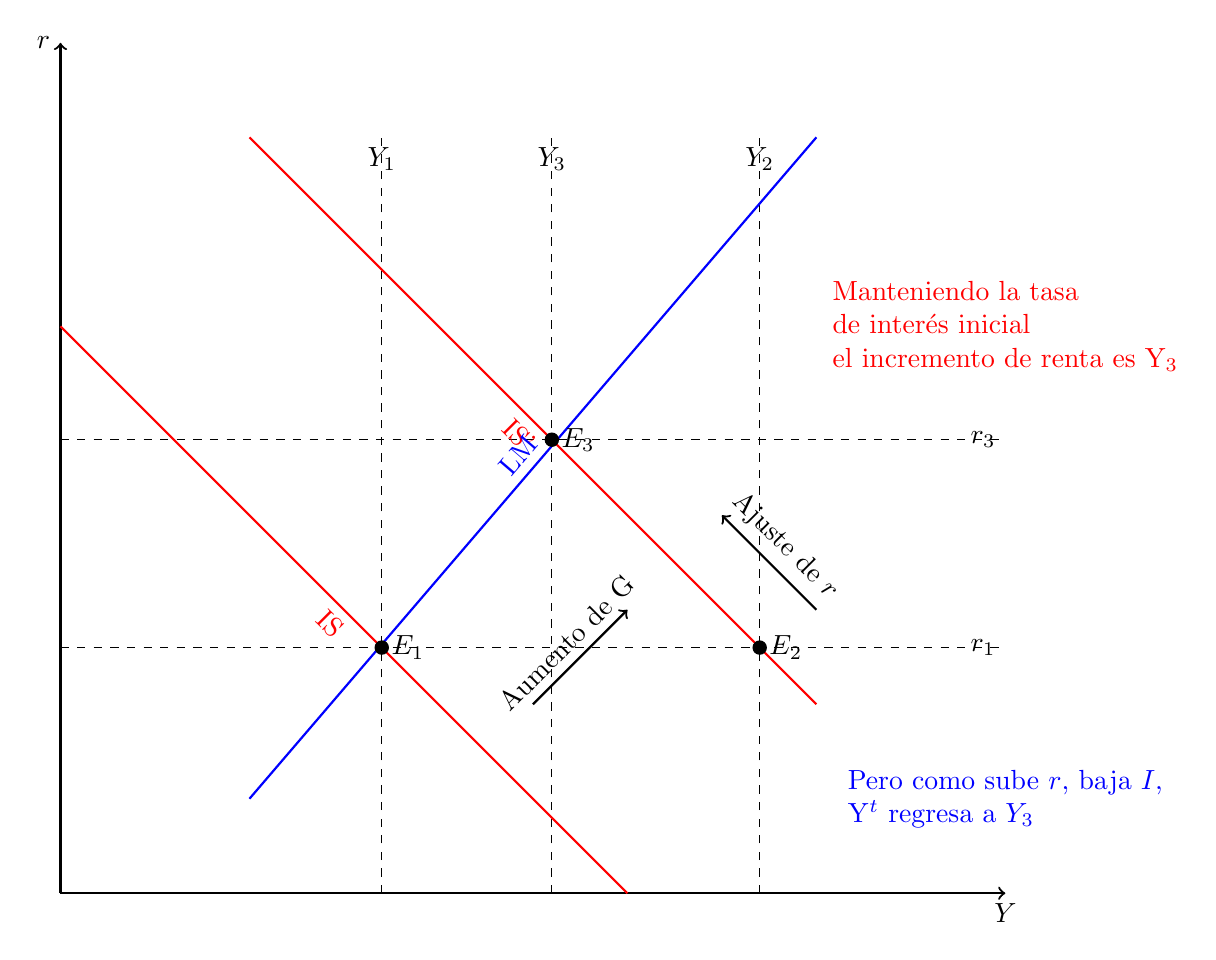
\begin{tikzpicture}[scale=1.2]
% Ejes
\draw[->, thick] (0,0) -- (10,0) node[below] {$Y$}; % Eje Y
\draw[->, thick] (0,0) -- (0,9) node[left] {$r$}; % Eje r
% Líneas de cuadrícula (punteadas)
\draw[dashed] (0,2.6) -- (10,2.6) node[left] {$r_1$};
\draw[dashed] (0,4.8) -- (10,4.8) node[left] {$r_3$};
\draw[dashed] (3.4,0) -- (3.4,8) node[below] {$Y_1$};
\draw[dashed] (5.2,0) -- (5.2,8) node[below] {$Y_3$};
\draw[dashed] (7.4,0) -- (7.4,8) node[below] {$Y_2$};
% Curva IS inicial
\draw[red, thick] (0,6) -- (6,0) node[midway, below, sloped] {IS};
% Curva IS desplazada
\draw[red, thick] (2,8) -- (8,2) node[midway, below, sloped] {IS'};
% Curva LM (pendiente positiva)
\draw[blue, thick] (2,1) -- (8,8) node[midway, above, sloped] {LM};
% Puntos de equilibrio
\filldraw (3.4,2.6) circle (2pt) node[right] {$E_1$}; % (Y_0, r_0), intersección IS y LM
\filldraw (7.4,2.6) circle (2pt) node[right] {$E_2$}; % (Y_2, r_1), en IS' con r_1 = r_0
\filldraw (5.2,4.8) circle (2pt) node[right] {$E_3$}; % (Y_3, r_2), intersección IS' y LM
% Flechas de desplazamiento
% Paralela a LM (pendiente positiva) para el desplazamiento de IS
\draw[->, thick] (5,2) -- (6,3) node[midway, above, sloped] {Aumento de \(\mathrm{G}\)};
% Paralela a IS (pendiente negativa) para el ajuste de r
\draw[->, thick] (8,3) -- (7,4) node[midway, above, sloped] {Ajuste de \(r\)};
% Anotaciones
\node[align=left, red] at (10,6) {Manteniendo la tasa \\ de interés inicial \\ el incremento de renta es \(\mathrm{Y}_3\) };
\node[align=left, blue] at (10,1) {Pero como sube \(r\), baja \(I\), \\ \(\mathrm{Y}^t\) regresa a \(Y_3\)};
\end{tikzpicture}
